\documentclass[dvisvgm]{standalone}

\usepackage{tikz}
\usetikzlibrary {arrows.meta, positioning, automata}

\begin{document}

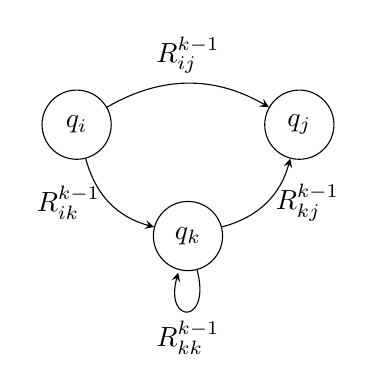
\begin{tikzpicture}[
    ->,
    >=stealth,
    node distance=2cm,
    initial text=$ $,
    on grid,
]

    \node[           state]                    (A) {$q_i$};
    \node[           state, below right =of A] (B) {$q_k$};
    \node[           state, above right =of B] (C) {$q_j$};

    \path
        (A) edge [above, bend left]       node {$R_{ij}^{k-1}$}  (C)  
        (A) edge [left, bend right]       node {$R_{ik}^{k-1}$}  (B)  
        (B) edge [right, bend right]      node {$R_{kj}^{k-1}$}  (C)  
        (B) edge [loop below]             node {$R_{kk}^{k-1}$}  (C)  
    ;
\end{tikzpicture}

\end{document}